%  %%%%%%%%%%%%%%Empieza la presentacion%%%%%%%%%%%%%%%%%%%%%%%%%%%%%%%%%%

\begin{frame}\frametitle{Señales aleatorias}
  
  \vspace{-0.2cm}
  
  \footnotesize
  
  \begin{itemize}
  \item Una señal aleatoria ($x(t)$ ó $x(n)$) es aquella cuyo comportamiento en cada instante de tiempo ($t$ ó $n$) se encuentra definido por una variable aleatoria asociada al instante de tiempo correspondiente ($X(t)$ ó $X(n)$).
  
  \item Al tener una variable aleatoria asociada a cada instante de tiempo, el comportamiento de la señal a lo largo del tiempo se puede definir
  
  \begin{columns}[c]
  \begin{column}{6cm}
  
  \begin{itemize}
  \footnotesize
  \item Con la función de probabilidad conjunta asociada a todas$^1$ las variables asociadas a la señal aleatoria
  \item A partir de un número infinito de secuencias muestrales.
  \item A partir de los estadísticos relacionados con las variables aleatorias
  \end{itemize}
  
  \end{column}
  \begin{column}{4cm}
  
  
  \color{olivegreen}$p(x(0),x(1),x(2),\dots,x(10))$
  
  \vspace{0.1cm}
  
  \hspace{0.2cm}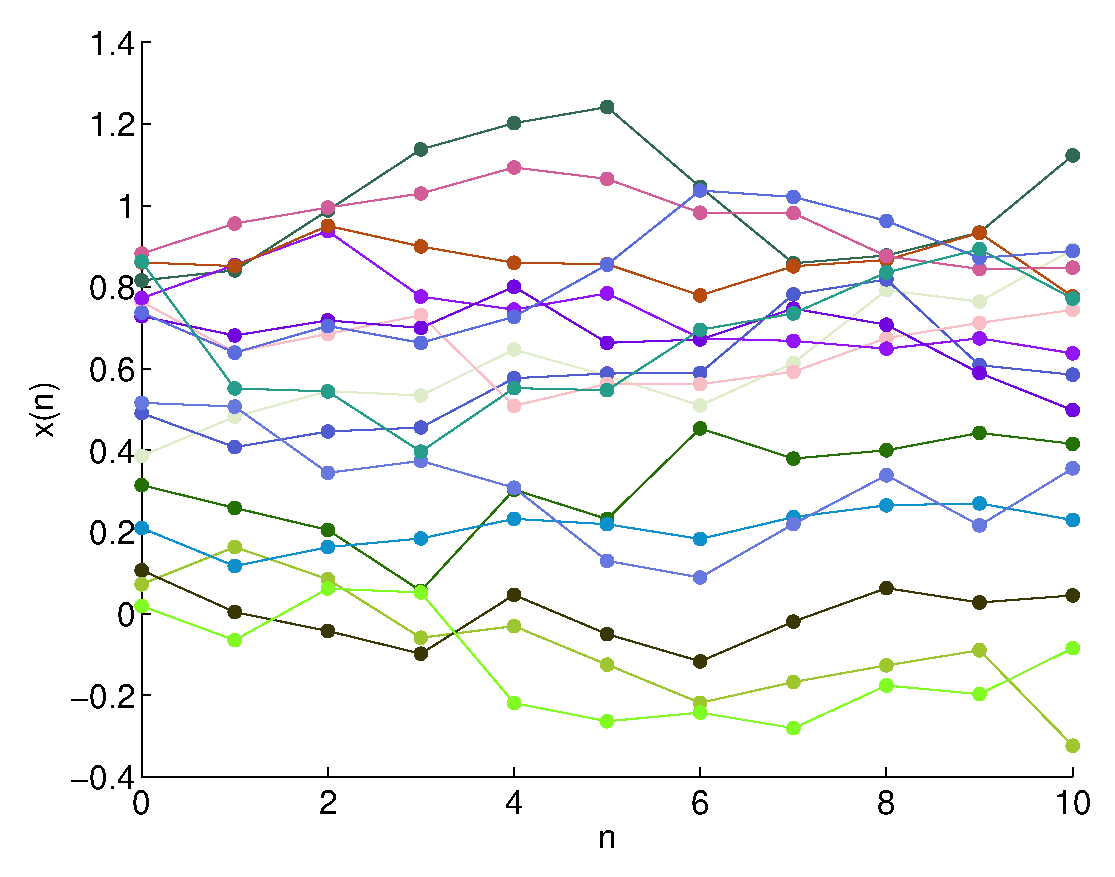
\includegraphics[width=3.5cm]{./Figures/SignalRandomDisc.eps}
  
  Ejemplos: $\mu_{x(n)}$, $\phi_{x(n)x(m)}$
  
  
  \end{column}
  \end{columns}
  
  
  \end{itemize}
  
  \rule{11cm}{0.04ex}
  \scriptsize
  
  $^1$ En principio, si la variable independiente es continua tendremos infinitas variables aleatorias, mientras que si la variable independiente es discreta tendremos tantas variables aleatorias como instantes de $n$ estemos analizando.
  
\end{frame}
  
  
  
\begin{frame}
\frametitle{Señales aleatorias}

\vspace{-0.2cm}

\footnotesize

\begin{itemize}
\item Una señal aleatoria ($x(t)$ ó $x(n)$) es aquella cuyo comportamiento en cada instante de tiempo ($t$ ó $n$) se encuentra definido por una variable aleatoria asociada al instante de tiempo correspondiente ($X(t)$ ó $X(n)$).

\item Al tener una variable aleatoria asociada a cada instante de tiempo, el comportamiento de la señal a lo largo del tiempo se puede definir

\begin{columns}[c]
\begin{column}{6cm}

\begin{itemize}
\footnotesize
\item Con la función de probabilidad conjunta asociada a todas$^1$ las variables asociadas a la señal aleatoria
\item A partir de un número infinito de secuencias muestrales.
\item A partir de los estadísticos relacionados con las variables aleatorias
\end{itemize}

\end{column}
\begin{column}{4cm}


\color{olivegreen}$p(x(0),x(1),x(2),\dots,x(10))$

\vspace{0.1cm}

\hspace{0.2cm}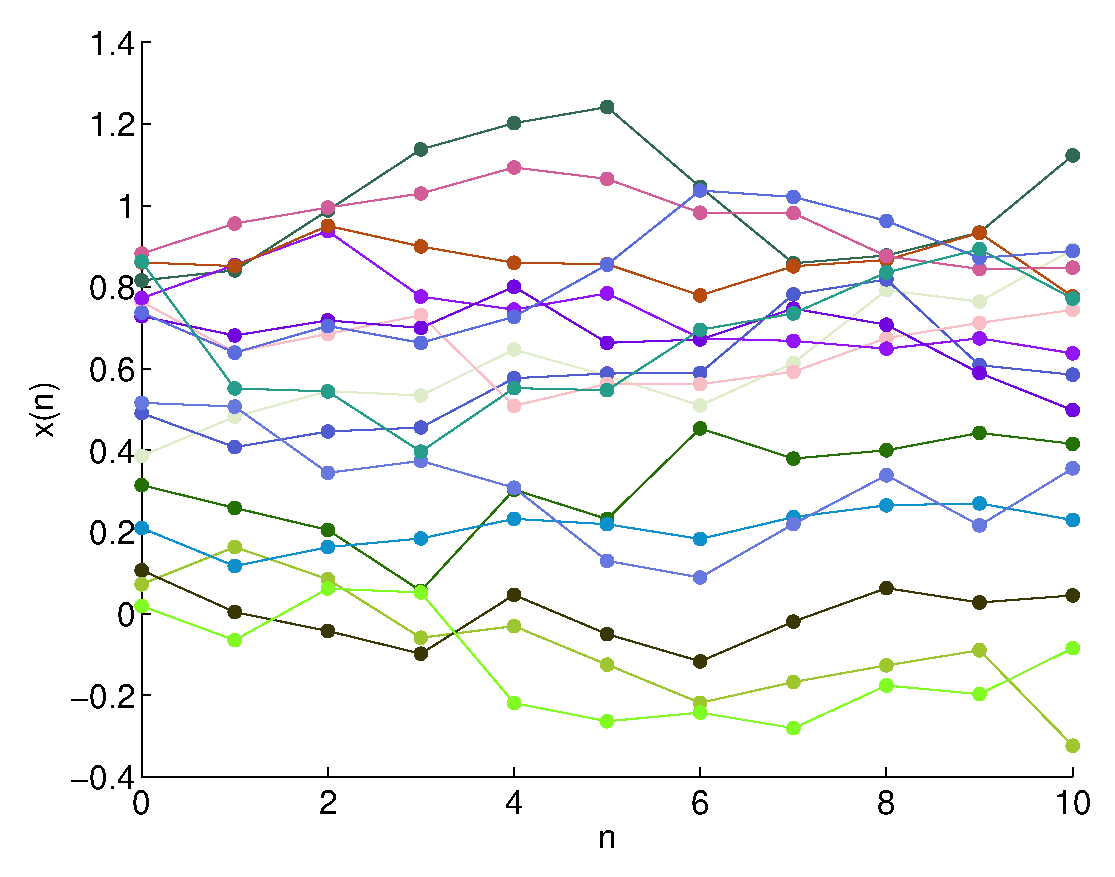
\includegraphics[width=3.5cm]{./Figures/SignalRandomDisc.eps}

Ejemplos: $\mu_{x(n)}$, $\phi_{x(n)x(m)}$


\end{column}
\end{columns}


\end{itemize}

\rule{11cm}{0.04ex}
\scriptsize

$^1$ En principio, si la variable independiente es continua tendremos infinitas variables aleatorias, mientras que si la variable independiente es discreta tendremos tantas variables aleatorias como instantes de $n$ estemos analizando.

\end{frame}

%%%%%%%%%%%%%%%%%%%%%%%%%%%%%%%%%%%%%%%%%%%%%%%%


\begin{frame}
\frametitle{Estadísticos de las señales aleatorias}

\vspace{-0.2cm}

\footnotesize

\begin{itemize}

\item Los estadísticos de una señal aleatoria, o de un par de señales aleatorias, se calculan de la misma forma que se calcula los estadísticos de conjuntos de variables aleatorias:
\begin{itemize}
\footnotesize
\item Probabilidades necesarias:

\begin{itemize}

\scriptsize

\item La probabilidad de la señal en cada instante: $p_{X(t)}(x(t))\triangleq p_X(x,t)$.

\item La probabilidad conjunta:

\hspace{0.2cm}De 1 señal en 2 instantes: $p_{X(t_1)X(t_2)}(x(t_1),x(t_2))\triangleq p_X(x_1,t_1,x_2,t_2)$.

\hspace{0.2cm}De 2 señales en 2 instantes: $p_{X_i(t_i)X_j(t_j)}(x_i(t_i),\!x_j(t_j))\!\triangleq \! p_{X_iX_j}(x_i,\!t_i,\!x_j,\!t_j)$.

\end{itemize}

\item Estadísticos habituales:

\begin{itemize}

\scriptsize

\item  Media: $\mu_X(t)\triangleq \mu_{X(t)}=\int_{-\infty}^\infty x(t)p(x(t))dx(t)=\int_{-\infty}^\infty xp(x,t)dx$

\item  Valor cuadrático medio: $\Psi_X(t)\triangleq  E(X^2(t))=\int_{-\infty}^\infty x^2(t)p(x(t))dx(t)=\int_{-\infty}^\infty x^2p(x,t)dx$

\item  Correlación cruzada: $\phi_{X_i,X_j}(t_i,t_j) \triangleq \phi_{X_i(t_i),X_j(t_j)}=\int_{-\infty}^\infty x_i(t_i)x_j(t_j)p(x_i(t_i),x_j(t_j))dx_i(t_i)dx_j(t_j)=\int_{-\infty}^\infty x_ix_jp(x_i,t_i,x_j,t_j)dx_idx_j$

\item Autocorrelación: $\phi_{XX}(t_1,t_2) \triangleq \phi_{X(t_1),X(t_2)}=\int_{-\infty}^\infty x(t_1)x(t_2)p(x(t_1),x(t_2))dx(t_1)dx(t_2)=\int_{-\infty}^\infty x_1x_2p(x_1,t_1,x_2,t_2)dx_1dx_2$

\end{itemize}

\end{itemize}
\end{itemize}


\rule{11cm}{0.04ex}
\scriptsize

Estas probabilidades se podrían obtener marginalizando de las conjuntas de la secuencia de la señal o de las secuencias de las señales las variables que no están involucradas en la probabilidad final.


\end{frame}


%%%%%%%%%%%%%%%%%%%%%%%%%%%%%%%%%%%%%%%%%%%%%%%%%


\begin{frame}
\frametitle{Tipos de señales aleatorias I}

\vspace{-0.2cm}

\footnotesize

\begin{itemize}
\item \alert{Señal Markoviana Discreta de Orden I: }

\begin{itemize}
\footnotesize
\item La probabilidad de la señal en un instante únicamente depende del valor de la variable en el instante anterior:  $p(x(n)|x(n-1))$

\vspace{0.1cm}

\visible<2->{

\item Este hecho permite realizar una factorización muy conveniente:
{\scriptsize

\vspace{0.1cm}

$p(x(0),x(1),\cdots,x(n))=$

\vspace{0.1cm}

\hspace{0.3cm}$=p(x(0)p(x(1)|x(0))p(x(2)|x(0),x(1))\cdots p(x(n)|x(0),\cdots,x(n-1))=$

\vspace{0.1cm}

\hspace{0.3cm}$=p(x(0))p(x(1)|x(0))p(x(2)|x(1))\cdots p(x(n)|x(n-1))=$

\vspace{0.1cm}

\hspace{0.3cm}$=p(x(0))\prod_{i=1}^n p(x(n)|x(n-1))$

}}
\end{itemize}


\end{itemize}



\visible<3->{

\color{olivegreen}Ejemplo: random walk gaussiano \color{gray}

\vspace{0.1cm}

{\scriptsize

\hspace{0.3cm}$p(x(0))=\mathcal{N}_X(x(0);1;0.1)$

\vspace{0.1cm}

\hspace{0.3cm}$p(x(n)|x(n-1))=\mathcal{N}_X(x(n);x(n-1);0.25)$ \visible<4->{$\rightarrow x(n)=x(n-1)+sqrt(0.25)*randn$}


}


\begin{columns}[c]
\begin{column}{6cm}

\vspace{-0.4cm}
\visible<5->{
\lstinputlisting{./Matlab/ProcMarkov.m}
}
\end{column}
\begin{column}{4cm}

\visible<6->{
\vspace{0.2cm}
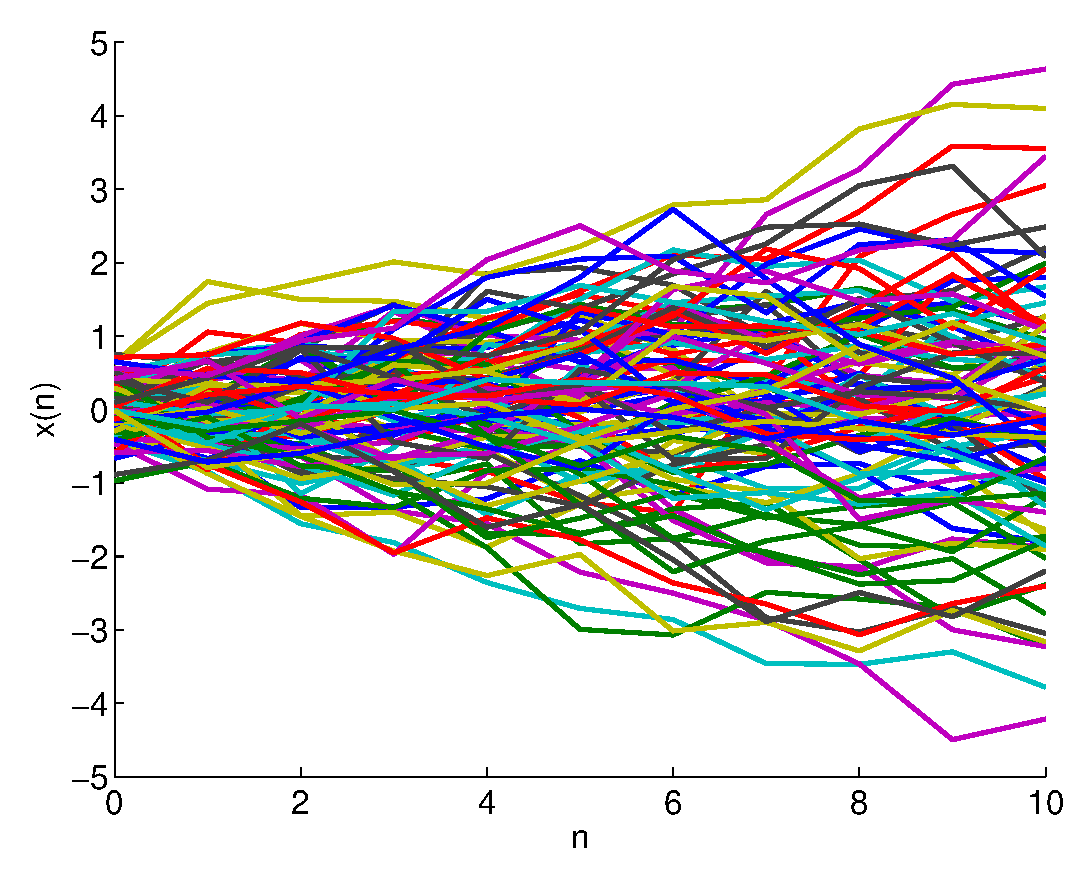
\includegraphics[width=3.5cm]{./Figures/RandomWalk.eps}
}
\end{column}
\end{columns}
}

\end{frame}

%%%%%%%%%%%%%%%%%%%%%%%%%%%%%%%%%%%%%%%%%%%%%%

\begin{frame}
\frametitle{Tipos de señales aleatorias II}


\footnotesize

\begin{itemize}
\item \alert{Señal Markoviana Continua de Orden I: }

\begin{itemize}
\footnotesize

\item Mientras que a la hora de modelar sistemas/señales discretos se utilizan los retardos para relacionar las variables, a la hora de modelar sistemas/señales continuos se utilizan las derivadas:

\vspace{0.1cm}
{
\color{olivegreen}
\hspace{0.5cm}Ejemplo discreto: $y(k)+y(k-1)+y(k-2)=x(k)$

\vspace{0.1cm}

\hspace{0.5cm}Ejemplo continuo: $\ddot y(t)+ \dot y(t) +y(t)=x(t)$

\vspace{0.1cm}

\color{black}}

\visible<2->{

\item Por lo tanto, la relación probabilística que se establece en señales Markovianas discretas entre una señal y su versión retardada, en señales Markovianas continuas se establece entre la derivada de la señal y la señal sin derivar:
  $p(\dot x(t)|x(t))$
}


\visible<3->{

\hspace{0.5cm}\color{olivegreen}Ejemplo: proceso Markov gaussiano \color{gray}

\vspace{0.1cm}




\scriptsize

\hspace{0.8cm}$p(x(0))=\mathcal{N}_X(x(0);1;0.1)$

\vspace{0.1cm}

\hspace{0.8cm}$p(\dot x(t)|x(t))\!=\!\mathcal{N}_X(\dot x(t);x(t);0.25)$

\vspace{0.1cm}

 \hspace{3.8cm}$\rightarrow \dot x(t)\!=\!x(t)\!+\!u(t)$ con $u(t)=\mathcal{N}_{U}(u,0,1)$

\hspace{0.8cm}Lo podríamos simular con lsim o Simulink, suponiendo un sistema de primer orden.

}

\end{itemize}
\end{itemize}

\end{frame}

%%%%%%%%%%%%%%%%%%%%%%%%%%%%%%%%%%%%%%%%%%%%%%

\begin{frame}
\frametitle{Tipos de señales aleatorias III}

\vspace{-0.2cm}

\footnotesize

\begin{itemize}
\item \alert{Señales aleatorias estacionarias (en sentido amplio): }
\begin{itemize}
\footnotesize

\visible<2->{
\item Son aquellas señales en las que la función de probabilidad no depende del tiempo: $p(x(t_1))=p(x(t_2))\triangleq p(x)$}

\vspace{0.1cm}

\visible<3->{

\item Este hecho implica que:

}

\begin{itemize}

\visible<3->{

\item Los estadísticos de una variable no dependen del tiempo:

\scriptsize

\vspace{0.1cm}

\hspace{0.2cm}Media: $\mu_X(t)\triangleq\int_{-\infty}^\infty x(t)p(x(t))dx(t)=\int_{-\infty}^\infty xp(x)dx= \alert{\mu_X}$


\vspace{0.1cm}

\hspace{0.2cm}Valor cuadrático medio:

\vspace{0.1cm}

\hspace{0.2cm}$\Psi_X(t)=\int_{-\infty}^\infty x^2(t)p(x(t))dx(t)=\int_{-\infty}^\infty x^2p(x)dx=\alert{\Psi_X}$

\vspace{0.1cm}

\hspace{0.2cm}Varianza: $\sigma^2_X(t)=\Psi_X(t)-\mu^2_X(t)=\Psi_X-\mu^2_X=\alert{\sigma^2_X}$


}

\vspace{0.1cm}

\visible<4->{
\footnotesize

\item Los estadísticos de dos variables dependen de la diferencia temporal:

\scriptsize

\vspace{0.1cm}

\hspace{0.2cm}Correlación cruzada:


\hspace{0.3cm}$\phi_{X_i,X_j}(t_i,t_j) =\int_{-\infty}^\infty x_i(t_i)x_j(t_j)p(x_i(t_i),x_j(t_j))dx_i(t_i)dx_j(t_j)=$

\hspace{0.4cm}$\int_{-\infty}^\infty x_i(t)x_j(t+\tau)p(x_i(t),x_j(t+\tau))dx_i(t)dx_j(t+\tau)=\alert{\phi_{X_iX_j}(\tau)}$

\vspace{0.1cm}

\hspace{0.2cm}Autocorrelación:

\hspace{0.3cm}$\phi_{XX}(t_1,t_2) =\int_{-\infty}^\infty x(t_1)x(t_2)p(x(t_1),x(t_2))dx(t_1)dx(t_2)=$

\hspace{0.4cm}$\int_{-\infty}^\infty x(t)x(t+\tau)p(x(t),x(t+\tau))dx(t)dx(t+\tau)=\alert{\phi_{XX}(\tau)}$
}
\end{itemize}

\end{itemize}
\end{itemize}
\end{frame}
%%%%%%%%%%%%%%%%%%%
\begin{frame}
\frametitle{Tipos de señales aleatorias IV}

\footnotesize

\vspace{-0.1cm}

\color{olivegreen}¿Cuales de las señales siguientes son estacionarias (en sentido amplio)?





%%%%%%%%%%%%%%%%%%%%%%%%

\begin{columns}[T]
\hspace{-0.5cm}\begin{column}{7cm}

\color{olivegreen}Ej1: ¿sistema discreto con variables $x(n)$ independientes y $p(x(n))=\mathcal{U}_{[a,b]}(x(n))$


 \color{gray}


\visible<2->{
\vspace{0.0cm}

Si, ya que las variables son independientes y tienen la misma función de probabilidad a lo largo del tiempo.
}
\end{column}
\begin{column}{2.5cm}
\visible<2->{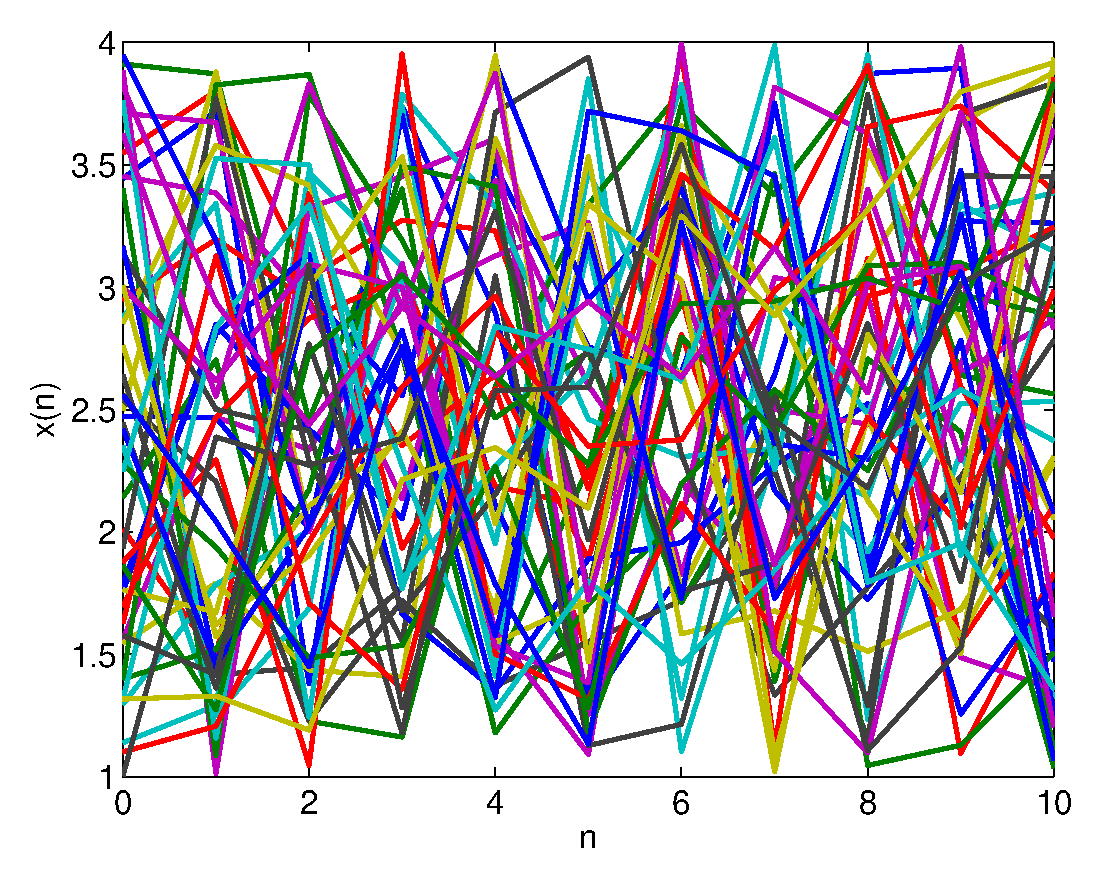
\includegraphics[width=2cm]{./Figures/Est1.eps}}
\end{column}
\end{columns}



%%%%%%%%%%%%%%%%%%%%%%%%%

\vspace{0.2cm}

\visible<3->{
\begin{columns}[T]
\hspace{-0.5cm}\begin{column}{7cm}




\color{olivegreen}Ej2: ¿sistema discreto con variables $x(n)$ independientes y $p(x(n))=\mathcal{N}_X(x(n);\mu_x,(0.5)^{n})$


 \color{gray}


\visible<4->{
\vspace{0.1cm}

No, ya que aunque las variables son independientes la función de probabilidad cambia a lo largo del tiempo.
}
\end{column}
\begin{column}{2.5cm}
\visible<4->{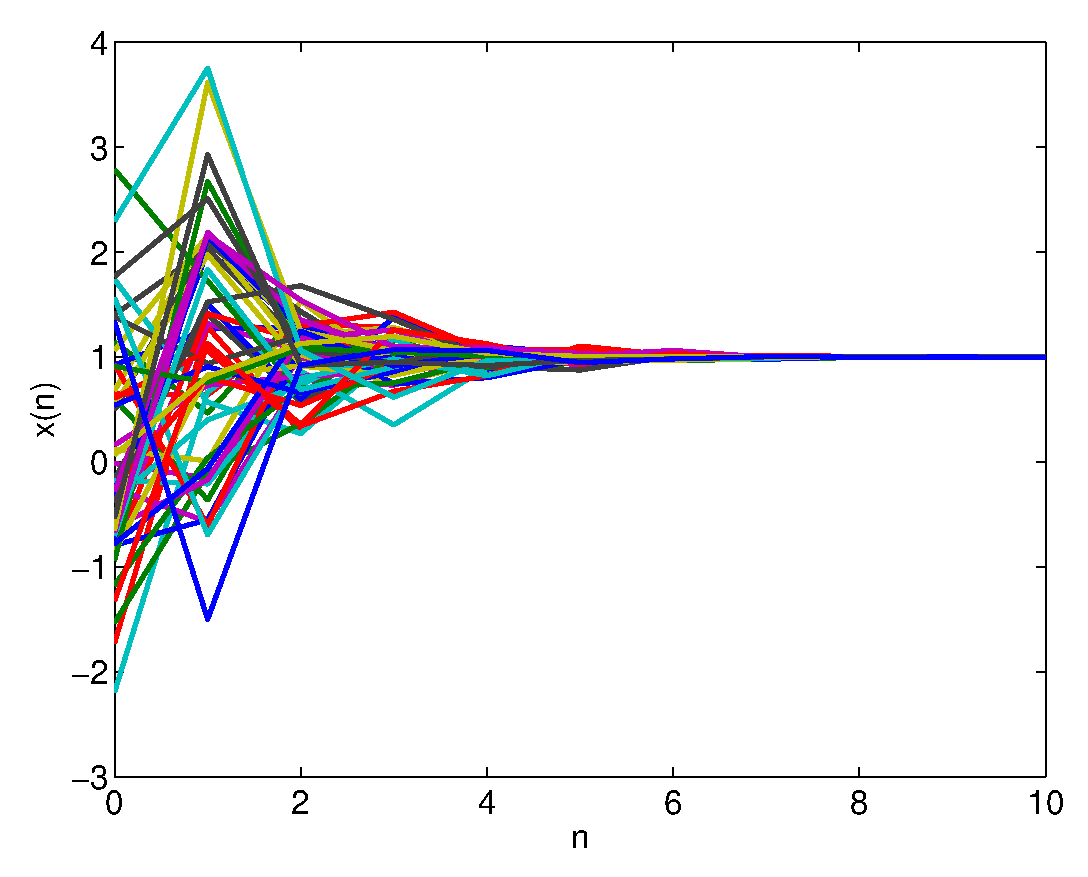
\includegraphics[width=2cm]{./Figures/Est2.eps} }
\end{column}
\end{columns}
}

%%%%%%%%%%%%%%%%%%%%%%%%%%%%%%%%%


\vspace{0.3cm}

\visible<5->{
\begin{columns}[T]
\hspace{-0.5cm}\begin{column}{7cm}

\color{olivegreen}Ej3: ¿random walk gaussiano discreto propuesto? \color{gray}


\visible<6->{
\vspace{-0.3cm}

No, ya que la varianza del proceso (estadístico de una variable) aumenta a lo largo del tiempo.
}
\end{column}
\begin{column}{2.5cm}
\visible<5->{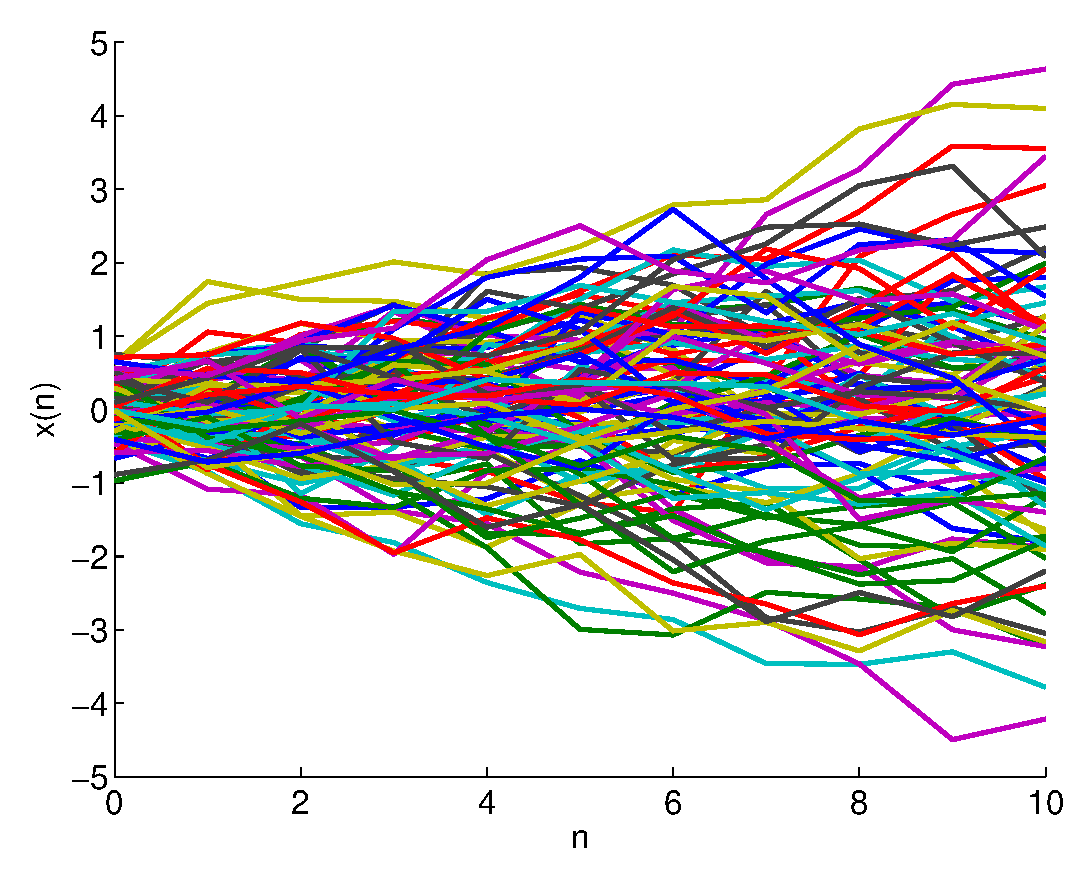
\includegraphics[width=2cm]{./Figures/RandomWalk.eps}}
\end{column}
\end{columns}

}

\vspace{0.1cm}

\visible<7->{
\begin{columns}[T]
\hspace{-0.5cm}\begin{column}{7cm}

\color{olivegreen}Ej4: Markoviano discreto $p(x(0))=U_{[a,b]}(x(0))$ y $p(x(n)|x(n-1))=\delta(x(n)-x(n-1))$  \color{gray}


\visible<8->{
\vspace{0.0cm}

Si, ya que se puede demostrar que $p(x(n))=U_{[a,b]}(x(n))$.
}
\end{column}
\begin{column}{2.5cm}
\visible<6->{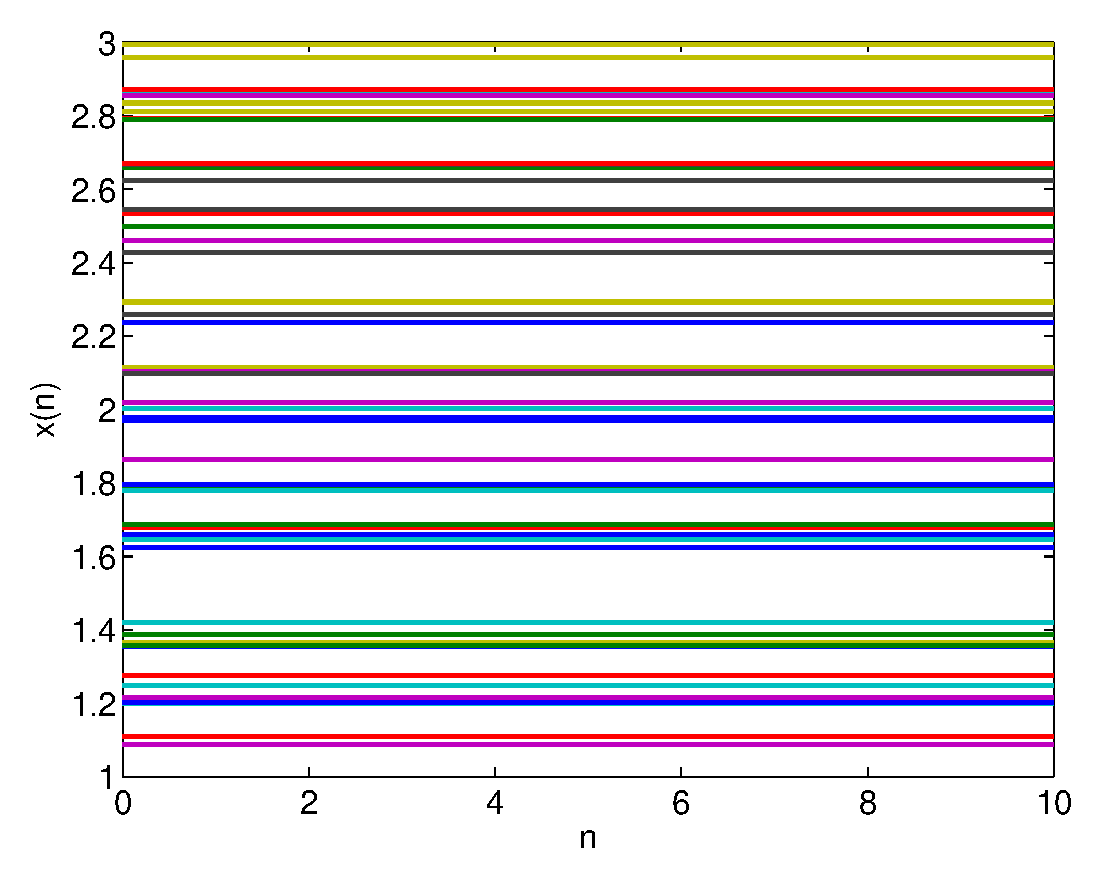
\includegraphics[width=2cm]{./Figures/Est3.eps}}
\end{column}
\end{columns}

}


\end{frame}

%%%%%%%%%%%%%%%%%%%%%%%%%%%%%%%%%%%%%%%%%%


\begin{frame}
\frametitle{Tipos de señales aleatorias V}

\vspace{-0.2cm}

\footnotesize

\begin{itemize}
\item \alert{Señales ergódicas: }
\begin{itemize}
\footnotesize
\item Son señales aleatorias \alert{estacionarias} cuyos estadísticos pueden ser caracterizados directamente a partir de una muestra (secuencia de valores) de la señal.

\visible<2->{
\item Es decir, en vez de tener que utilizar la función de probabilidad conjunta o las infinitas muestras de la señal en cada  instante de tiempo, los estadísticos se pueden estimar a partir de los valores de una muestra de la señal real.
}

\visible<3->{
\item La redefinición de los estadísticos a partir de una muestra (secuencia de valores) de la señal no requiere de funciones de probabilidad, si no del cálculo de la media, ... y correlación de las señales directamente:

\begin{itemize}
\scriptsize

\item Media: $\mu_X \triangleq \lim_{T \rightarrow \infty} \frac{1}{2T}\int_{-T}^T x(t)dt$


\vspace{0.1cm}

\item Valor cuadrático medio: $\Psi_X \triangleq \lim_{T \rightarrow \infty} \frac{1}{2T} \int_{-T}^T x^2(t)dt$


\vspace{0.1cm}

\item Correlación cruzada: $\phi_{X_i,X_j}(\tau)  \triangleq \lim_{T \rightarrow \infty} \frac{1}{2T}\int_{-T}^T x_i(t)x_j(t+\tau)dt$

\item Autocorrelación: $\phi_{XX}(\tau) \triangleq \lim_{T \rightarrow \infty} \frac{1}{2T}\int_{-T}^T x(t)x(t+\tau)dt$

\end{itemize}
}

\end{itemize}
\end{itemize}

\end{frame}

%%%%%%%%%%%%%%%%%%%%%%%%%

%%%%%%%%%%%%%%%%%%%%%%%%%%%%%%%%%%%%%%%%%%


\begin{frame}
\frametitle{Tipos de señales aleatorias VI}

\footnotesize

\vspace{-0.1cm}

\color{olivegreen}¿Cuales de las señales siguientes son ergódicas?





%%%%%%%%%%%%%%%%%%%%%%%%

\begin{columns}[T]
\hspace{-0.5cm}\begin{column}{7cm}

\color{olivegreen}Ej1: ¿sistema discreto con variables $x(n)$ independientes y $p(x(n))=\mathcal{U}_{[a,b]}(x(n))$


 \color{gray}


\visible<2->{
\vspace{0.0cm}

Si, ya que es estacionario y se puede obtener los estadísticos de una única secuencia de valores.
}
\end{column}
\begin{column}{2.5cm}
\visible<2->{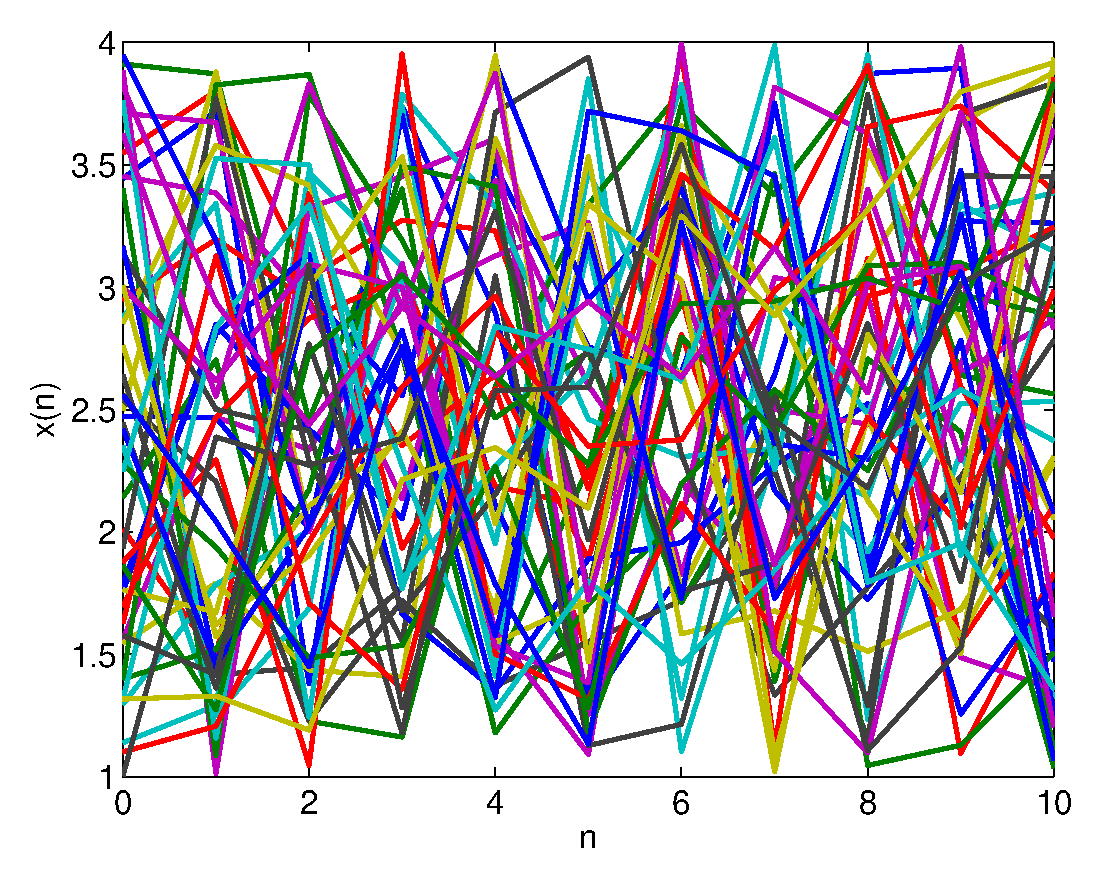
\includegraphics[width=2cm]{./Figures/Est1.eps}}
\end{column}
\end{columns}



%%%%%%%%%%%%%%%%%%%%%%%%%

\vspace{0.2cm}

\visible<3->{
\begin{columns}[T]
\hspace{-0.5cm}\begin{column}{7cm}




\color{olivegreen}Ej2: ¿sistema discreto con variables $x(n)$ independientes y $p(x(n))=\mathcal{N}_X(x(n);\mu_x,(0.5)^{n})$


 \color{gray}


\visible<4->{
\vspace{0.1cm}

No, ya que no es estacionario.
}
\end{column}
\begin{column}{2.5cm}
\visible<4->{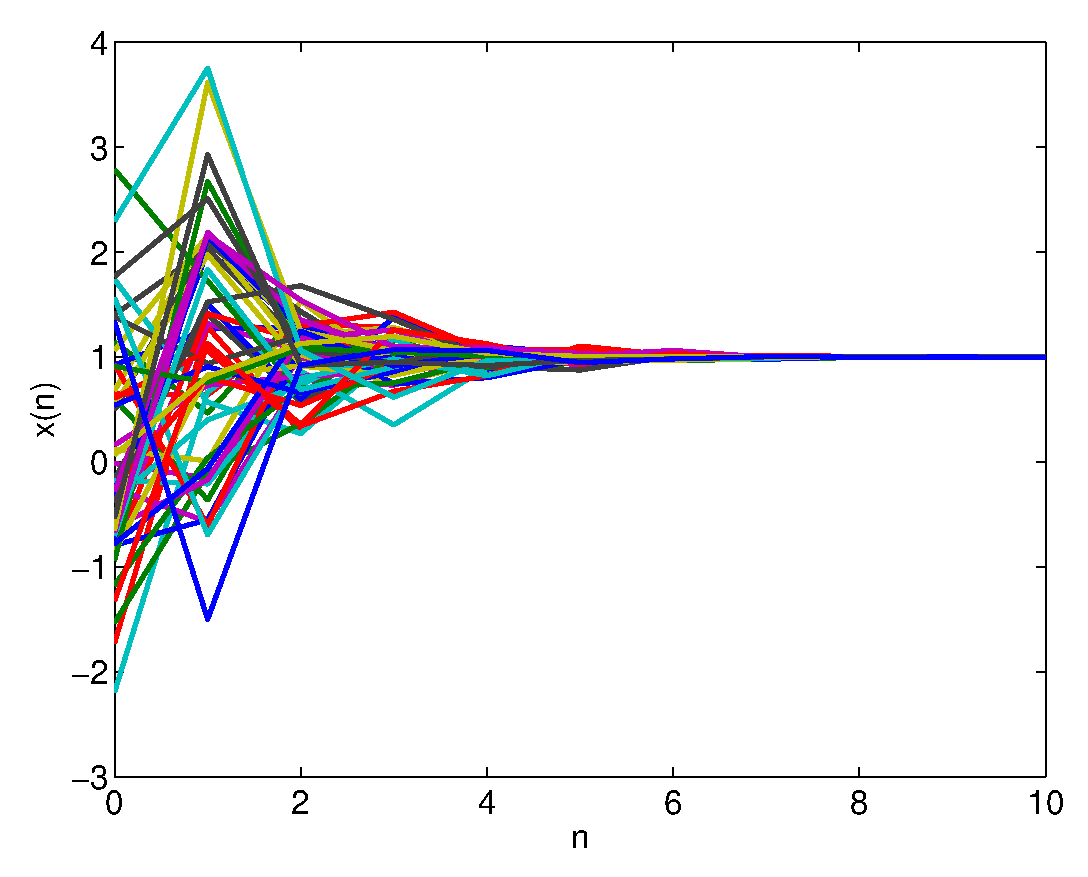
\includegraphics[width=2cm]{./Figures/Est2.eps} }
\end{column}
\end{columns}
}

%%%%%%%%%%%%%%%%%%%%%%%%%%%%%%%%%


\vspace{0.3cm}

\visible<5->{
\begin{columns}[T]
\hspace{-0.5cm}\begin{column}{7cm}

\color{olivegreen}Ej3: ¿random walk gaussiano discreto propuesto? \color{gray}


\visible<6->{
\vspace{-0.3cm}

No, ya que no es estacionario.
}
\end{column}
\begin{column}{2.5cm}
\visible<5->{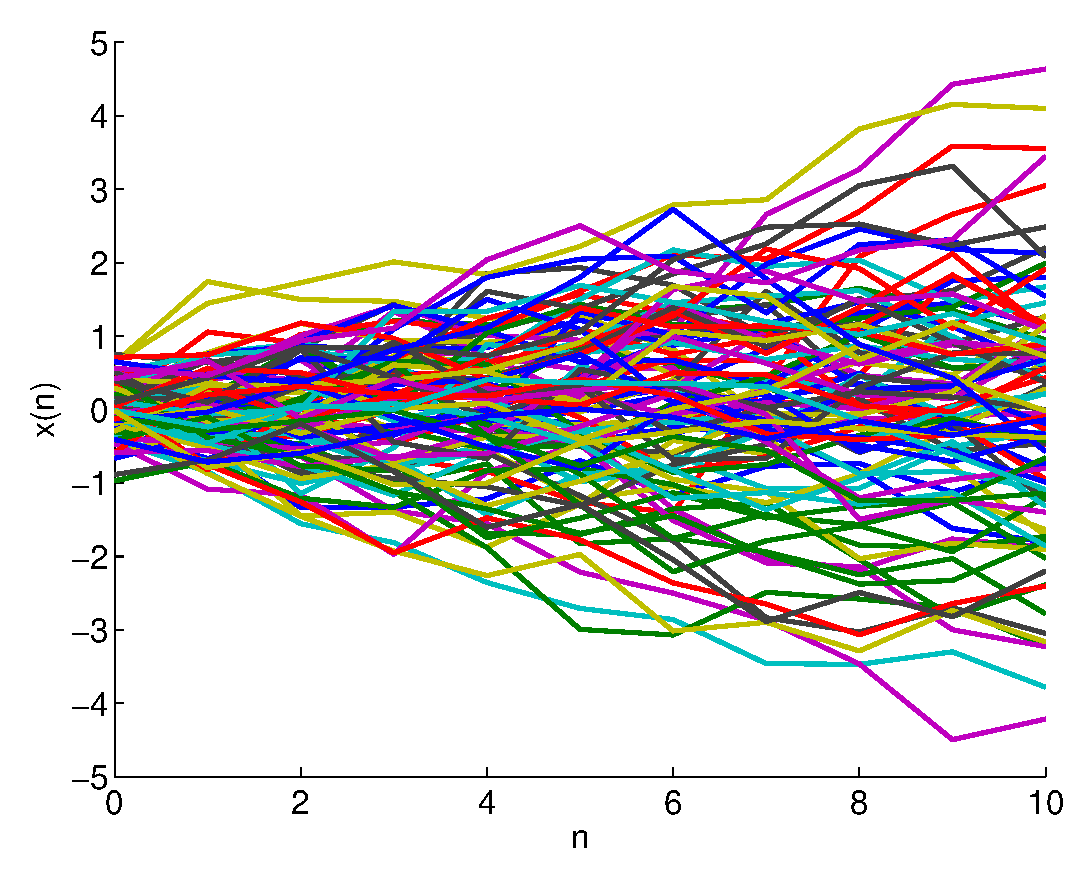
\includegraphics[width=2cm]{./Figures/RandomWalk.eps}}
\end{column}
\end{columns}

}

\vspace{0.1cm}

\visible<7->{
\begin{columns}[T]
\hspace{-0.5cm}\begin{column}{7cm}

\color{olivegreen}Ej4: Markoviano discreto $p(x(0))=U_{[a,b]}(x(0))$ y $p(x(n)|x(n-1))=\delta(x(n)-x(n-1))$  \color{gray}


\visible<8->{
\vspace{0.0cm}

No, ya que una secuencia de valores no es representativa de la muestra (cada señal toma un valor constante).
}
\end{column}
\begin{column}{2.5cm}
\visible<6->{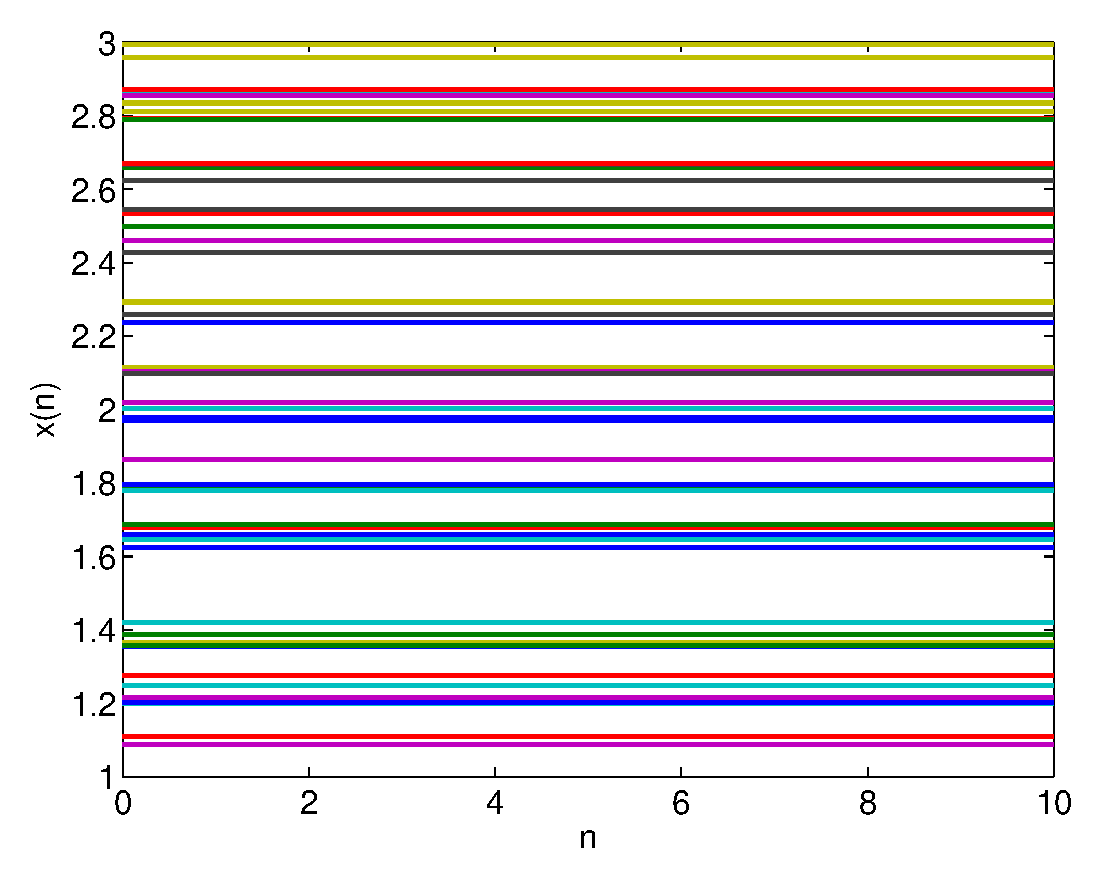
\includegraphics[width=2cm]{./Figures/Est3.eps}}
\end{column}
\end{columns}

}

\end{frame}





%%%%%%%%%%%%%%%%%%%%%%



\begin{frame}
\frametitle{Señales aleatorias estacionarias: Propiedades I}

\footnotesize

\begin{itemize}

\item Media ($\mu_X$), Valor cuadrático medio ($\Psi_X$), y la varianza $\sigma_X^2$ son constantes en el tiempo.
\item Correlación cruzada ($\phi_{XY}(\tau)$), autocorrelacion ($\phi_{XX}(\tau)$) y covarianza cruzada ($\phi_{XY}(\tau)$) dependen de la diferencia temporal $\tau$.

\item Relaciones con la autocorrelación:


\begin{itemize}

\footnotesize

\item La autocorrelación en el instante inicial es igual al valor cuadrático medio: $\phi_{XX}(0)=\Psi_X=E(X^2)$.

{\scriptsize
\color{gray}

$\Psi_X=E(X^2)=\int x^2(t) p(x(t))dx(t)$

$\phi_{XX}(\tau)=\int x(t)x(t+\tau) p(x(t),x(t+\tau))dx(t)$
}

\item $\phi_{XX}(\infty)=|\mu_X|^2.$

\item $\phi_{XX}(0)>\phi_{XX}(\tau)$  (el máximo de la autocorrelación está en cero)

\item Estas propiedades nos pueden permitir saber si la señal tiene una componente determinista o no:

\begin{itemize}

\item Si no la tiene deberá tender al valor medio según pasa el tiempo.
\item Si la tiene  la autocorrelación tendrá un comportamiento diferente.
\item Aun más, en el caso en que la señal tenga un comportamiento determinista periódico, la autocorrelación también mostrará el comportamiento periódico.
\end{itemize}
\end{itemize}
\end{itemize}


\end{frame}

%%%%%%%%%%%%%%%%%%%%%%%%%%%%%%%%%%%%%%%%%%%%%%%

\begin{frame}
\frametitle{Señales aleatorias estacionarias: Propiedades II}

\footnotesize

\vspace{-0.1cm}

\color{olivegreen}Ejemplos de autocorrelación de señales ergódicas (usadas como casos de estacionarias porque permiten cálculos a partir de una secuencia de valores).

\begin{itemize}

\scriptsize
\item \color{blue}\texttt{[phixy,lags]=xcorr(x,y,limk,'unbiased')}: \color{black}cálculo de la correlación$^1$ cruzada de las señales x e y.
\item \color{blue}\texttt{[phixy,lags]=xcorr(x,limk,'unbiased')}: \color{black} cálculo de la autocorrelación$^1$ de la señal x.

\end{itemize}

%%%%%%%%%%%%%%%%%%%%%%%%

\visible<2->{

\begin{columns}[T]
\hspace{-0.5cm}\begin{column}{6cm}

\color{olivegreen}Ej1: Sistema continuo con variables $x(t)$ independientes y $p(x(t))=\mathcal{N}(x(t);5,1)$

\color{black}

\vspace{0.1cm}

Lo discretizamos con periodo $T_s=0.01$

\vspace{-0.3cm}

\lstinputlisting{./Matlab/Auto1.m}

\end{column}
\begin{column}{4cm}
\visible<3->{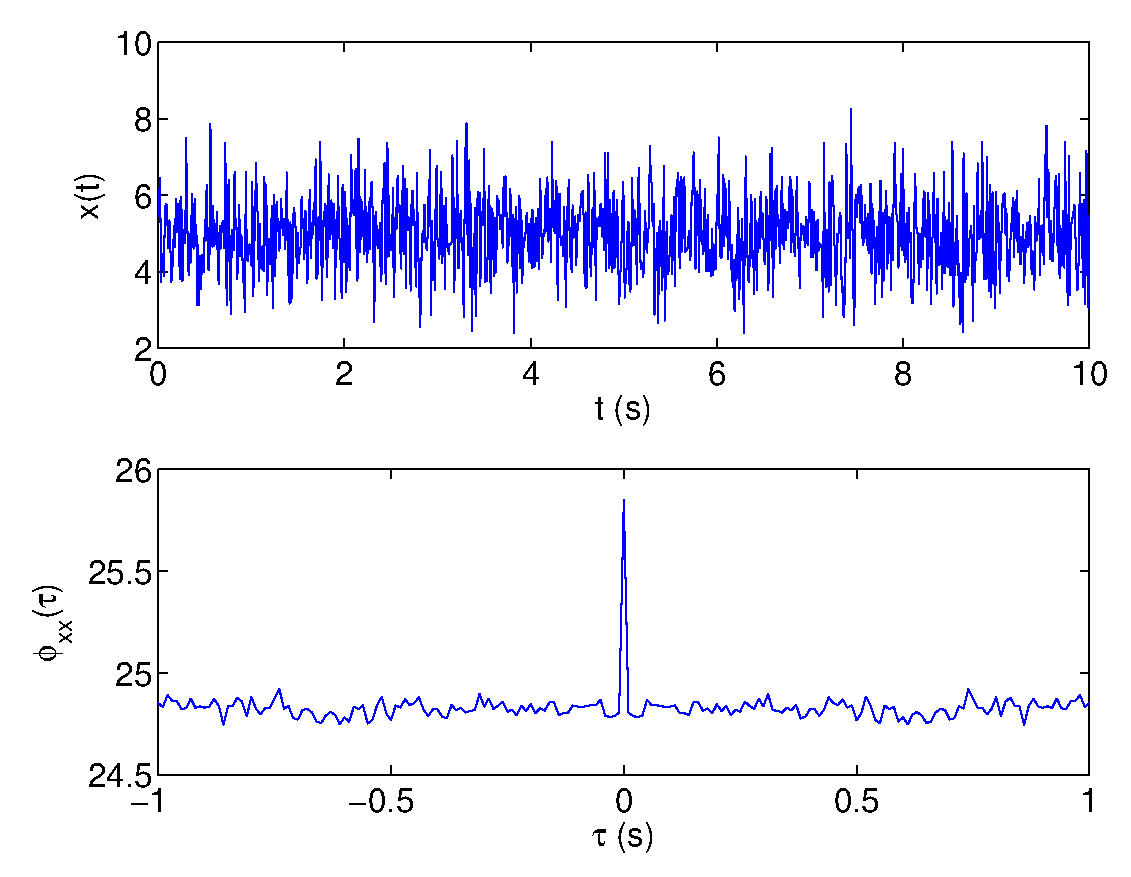
\includegraphics[width=3.2cm]{./Figures/Auto1.eps}

\scriptsize
\color{gray}
$\phi_{XX}(0)=\Psi_X=\sigma^2_X+\mu^2_X=26$

$\phi_{XX}(\infty) \rightarrow \mu^2_X=25$}



\end{column}
\end{columns}

}

\rule{11cm}{0.04ex}
\scriptsize

$^1$\color{blue}\texttt{liml } \color{black} se utiliza para limitar los valores de la $k$ sobre los que se calcula la correlación y la autocorrelación. Los límites temporales están $\tau=\pm T_s limk$.

\end{frame}

%%%%%%%%%%%%%%%%%%%%%%%%%

\begin{frame}

\frametitle{Señales aleatorias estacionarias: Propiedades III}

\footnotesize

\vspace{-0.1cm}

\begin{columns}[T]
\hspace{-0.5cm}\begin{column}{6cm}

\color{olivegreen}Ej2: Sistema continuo con variables $x(t)$ independientes y $p(x(t))=\mathcal{U}_{[2,6]}(x(t))$

\color{black}

\vspace{0.1cm}

Lo discretizamos con periodo $T_s=0.01$


\vspace{-0.3cm}

\lstinputlisting{./Matlab/Auto2.m}

\end{column}
\begin{column}{4cm}
\visible<2->{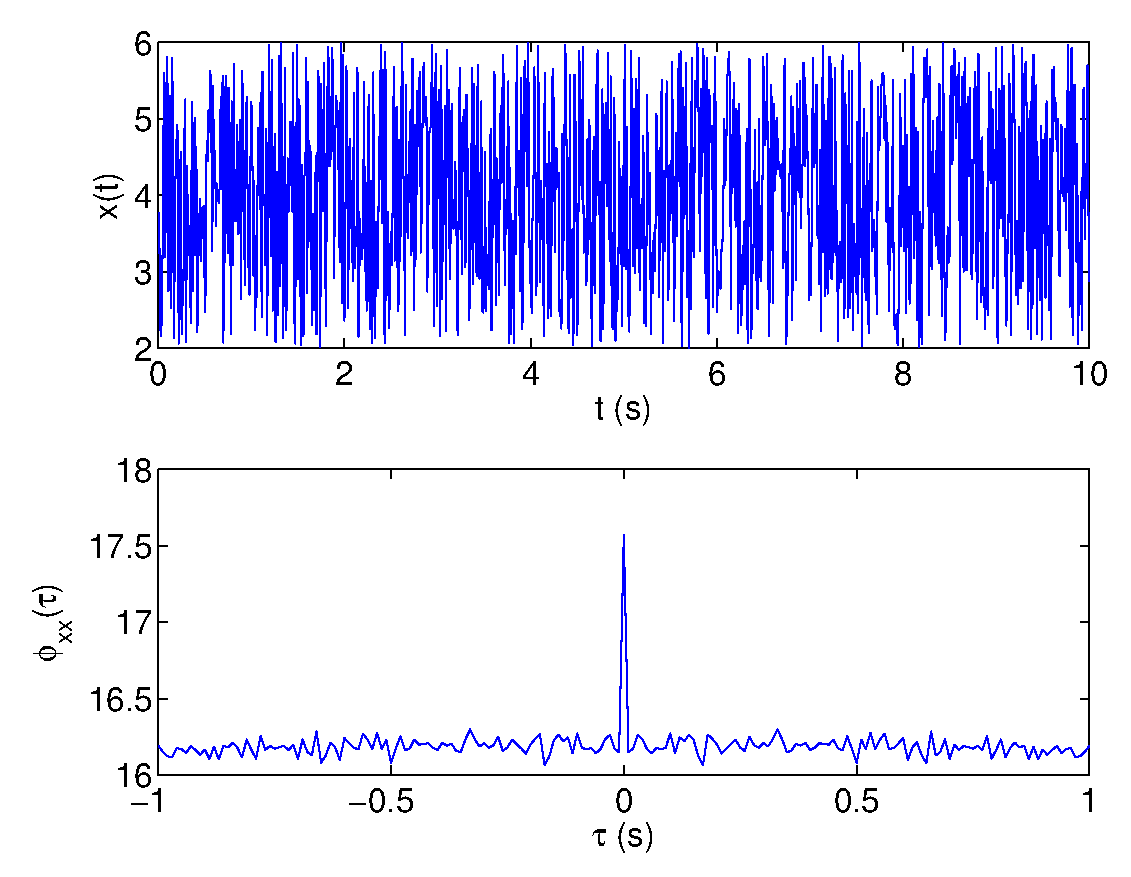
\includegraphics[width=3.2cm]{./Figures/Auto2.eps}

\scriptsize
\color{gray}
$\phi_{XX}(0)\!=\!\Psi_X\!=\!\frac{b^2+a^2+ab}{3}\!=\!17.3$

$\phi_{XX}(\infty) \rightarrow \mu^2_X=\left(\frac{b+a}{2}\right )^2=16$}

\end{column}
\end{columns}


%%%%%%%%%%%%%%%%%%%%%%%%%%%%%%%%%%%%%%%%%%
\vspace{0.3cm}

\visible<3->{
\begin{columns}[c]
\hspace{-0.5cm}\begin{column}{6cm}

\color{olivegreen}Ej3: Sistema continuo determinista con $x(t)=sen(2\pi F t)$ con $F=10$ Hz.

\color{black}

\vspace{0.1cm}

Lo discretizamos con periodo $T_s=0.01$


\vspace{-0.3cm}

\lstinputlisting{./Matlab/Auto3.m}

\end{column}
\begin{column}{4cm}
\visible<4->{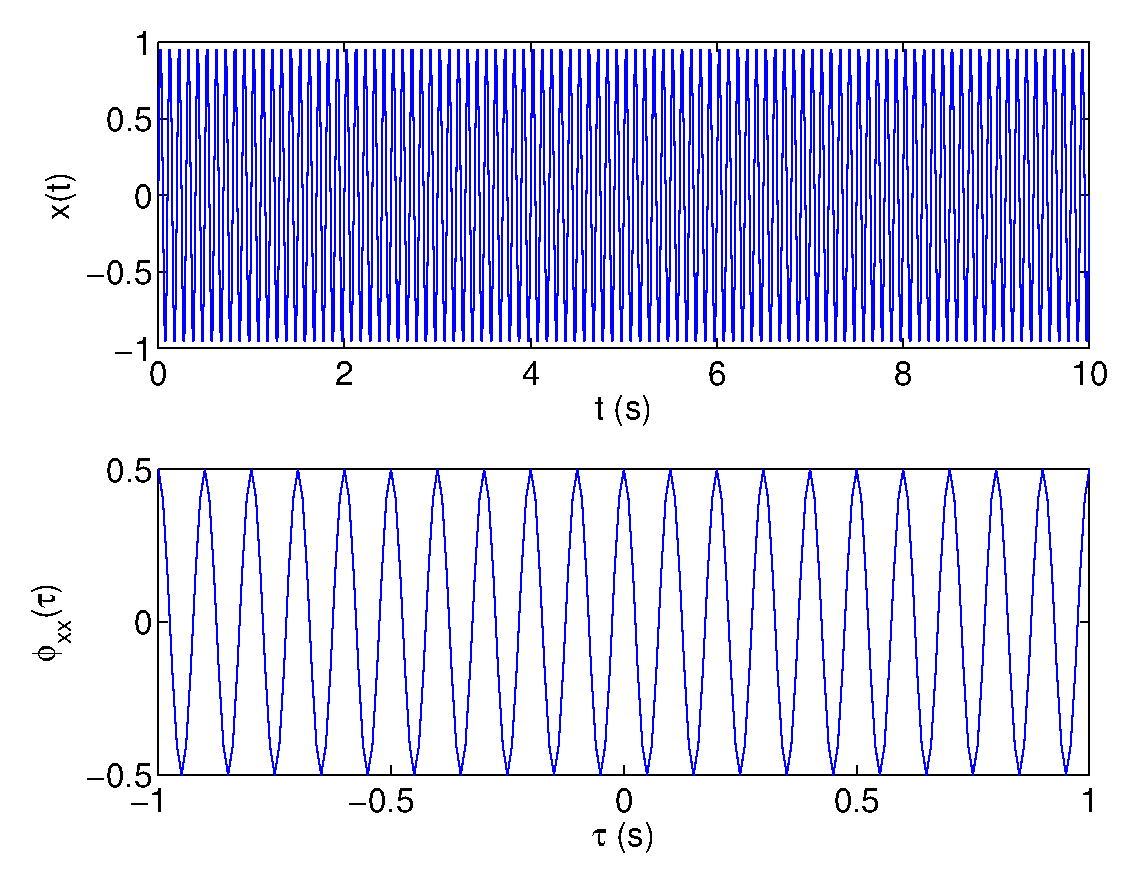
\includegraphics[width=4cm]{./Figures/Auto3.eps}}




\end{column}
\end{columns}}

\end{frame}


%%%%%%%%%%%%%%%%%%%%%%%%%%%%%%%%%%%%%%%%%%%%%%%%

\begin{frame}
\frametitle{Señales aleatorias estacionarias: Propiedades IV}


\footnotesize
\begin{itemize}

\item Relaciones con la correlación cruzada:


\begin{itemize}

\footnotesize

\item No tiene necesariamente un máximo en $\tau=0$

\vspace{0.1cm}

\item $\phi_{XY}(\tau)=\phi_{YX}(-\tau)$

\vspace{0.1cm}

\item  $|\phi_{XY}(\tau)|^2 \le \phi_{XX}(0) \phi_{YY}(0)$

\vspace{0.1cm}

\item  $|\phi_{XY}(\tau)| \le \frac{1}{2} [\phi_{XX}(0) +\phi_{YY}(0)]$

\vspace{0.1cm}

\item  Si las variables son independientes $\phi_{XY}(0)=\mu_X \mu_Y$.

\end{itemize}


\item Utilidades adicionales de la función de correlación cruzada:

\begin{itemize}

\footnotesize

\item Determinar retardos entre señales: esto se debe a que en la zona en la que se superpongan la señal original y la señal retardada aparece un máximo en la señal de correlación cruzada. A veces el pico no es lo suficientemente significativo para para poder determinar el retardo.

\item Determinación de caminos de transmisión con diferentes retardos.

\item Recuperar señales con ruido (podemos calcular la correlación de la señal original sin ruido con la que viene con ruido y determinar los picos donde se superponen).

\end{itemize}

\end{itemize}
\end{frame}

%%%%%%%%%%%%%%%%%%%%%%%%%%%%%%%%%%%%%%%%
\begin{frame}
\frametitle{Señales aleatorias estacionarias: Propiedades V}

\footnotesize


\color{olivegreen}Ejemplos de aplicación de correlación cruzada de señales.

%%%%%%%%%%%%%%%%%%%%%%%%

\vspace{0.2cm}

\begin{columns}[T]
\hspace{-0.3cm}\begin{column}{6cm}

\color{olivegreen}Ej1: Calcular el desfase de las señales $x(t)=sinc(t-2)$ y $y(t)=sinc(t-3)$

\color{black}

\vspace{0.1cm}

Lo discretizamos con periodo $T_s=0.01$

\vspace{-0.4cm}

\lstinputlisting{./Matlab/Corr1.m}

\end{column}
\begin{column}{4cm}
\visible<2->{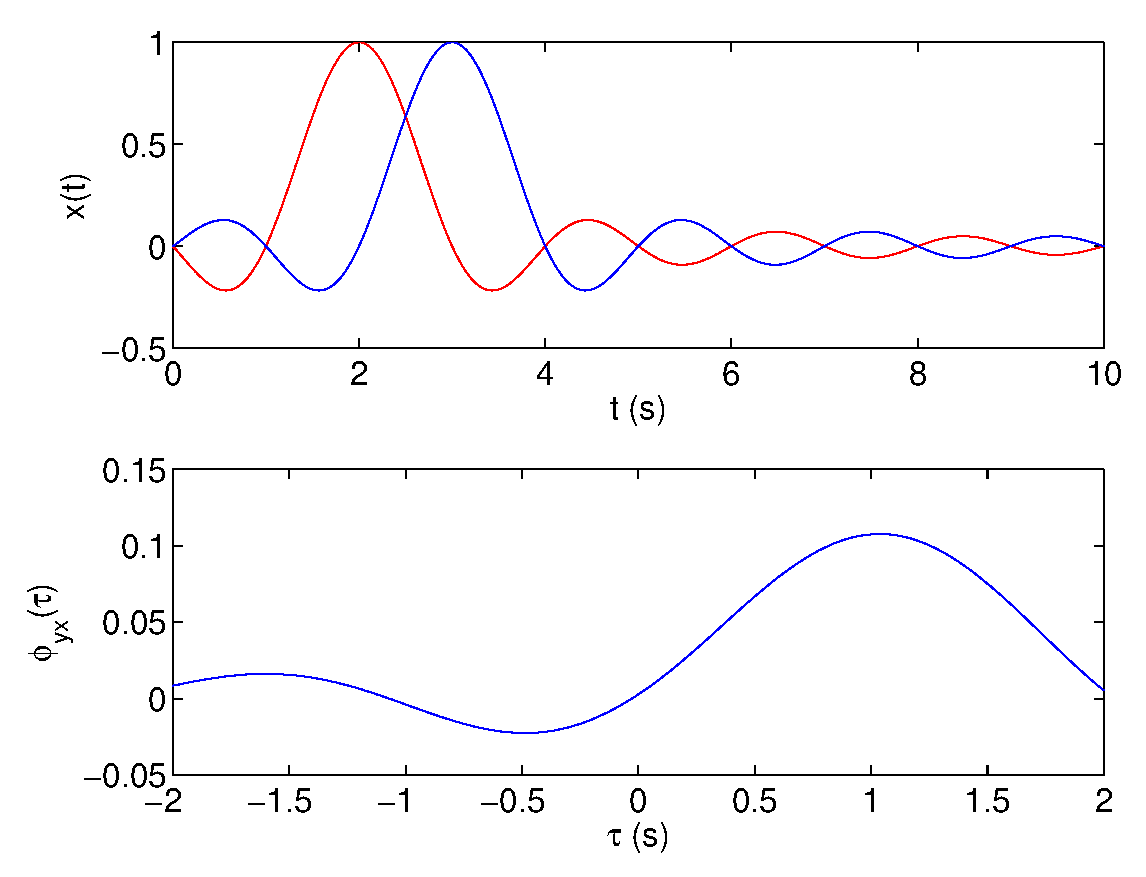
\includegraphics[width=3.2cm]{./Figures/CrossCorr1.eps}

\scriptsize
\color{gray}
Máximo en $\tau=1$, tiempo que está retardada la señal.
}



\end{column}
\end{columns}
\visible<3->{

\vspace{0.2cm}

\begin{columns}[T]
\hspace{-0.35cm}\begin{column}{6cm}

\color{olivegreen}Ej2: Localizar la señal $x(t)=sinc(t-2)$ en $y(t)=sinc(t-3)+u(t)$ con $u(t)\sim \mathcal{N}_U(u,0,4)$

\color{black}

\vspace{0.1cm}

Lo discretizamos con periodo $T_s=0.01$

\vspace{-0.4cm}

\lstinputlisting{./Matlab/Corr2.m}

\end{column}
\begin{column}{4cm}
\visible<4->{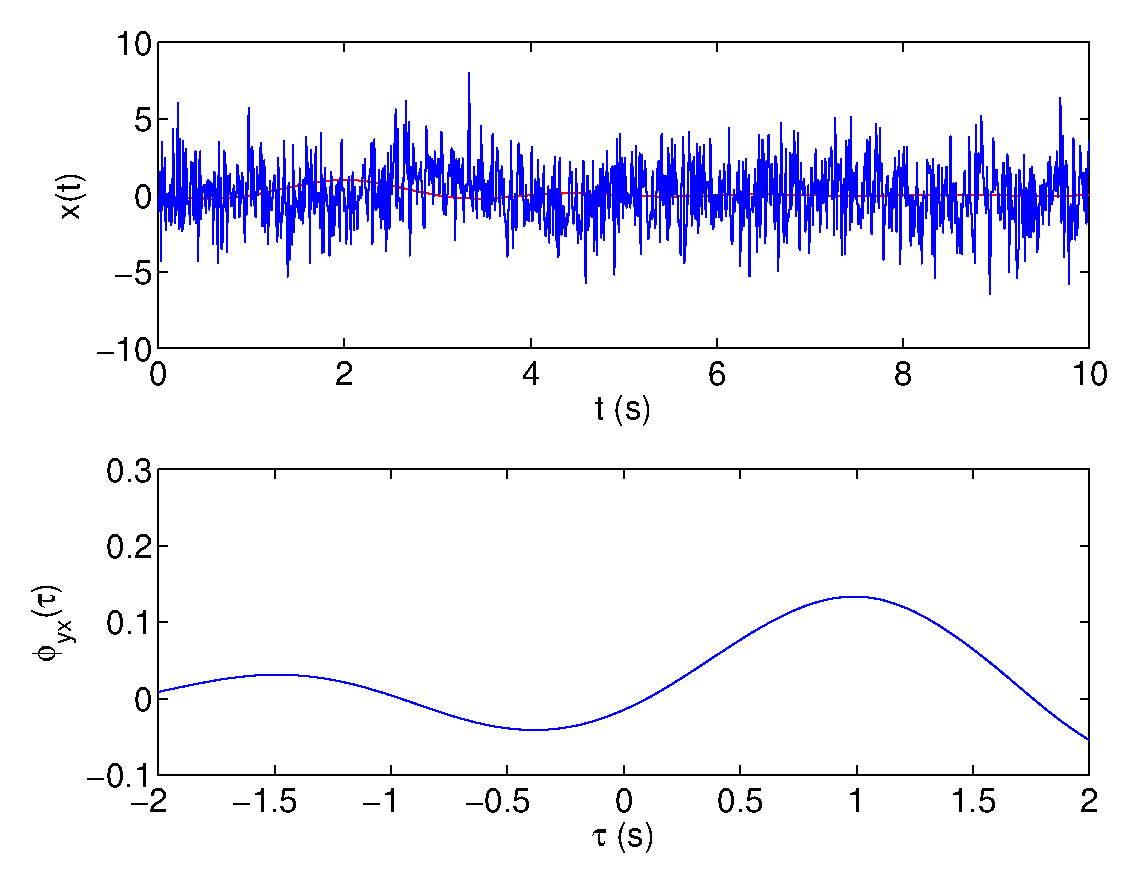
\includegraphics[width=3.2cm]{./Figures/CrossCorr2.eps}

\scriptsize
\color{gray}
Máximo en $\tau=1$,  tiempo que está retardada la señal determinista buscada
}


\end{column}
\end{columns}
}


\end{frame}
